% Dieses sheet hat nur die Aufgaben, das heißt es beginnt erst nach der inhaltlichen Präsi, wo schon alle Internet und intelliJ haben sollten.
\documentclass{../../sheet}
\renewcommand{\logopath}{../../logos/}

\title{PSE Vorkurs Tag 1}

\begin{document}
\maketitle

\aufgabe{Wichtige Shortcuts:}
\begin{enumerate}
    \item Code automatisch formattieren (z.B. richtig Einrücken): \textbf{Strg+Alt+L}
    \item Code kopieren: \textbf{Strg+C}
    \item Mit \textbf{Strg+C} kopierten Code woanders einfügen: \textbf{Strg+V}
    \item Letzte Aktion rückgängig machen: \textbf{Strg+Z}
    \item IntelliJ Autovervollständigungsvorschläge annehmen (siehe Bild): \textbf{Tab}
    
    \begin{center}
        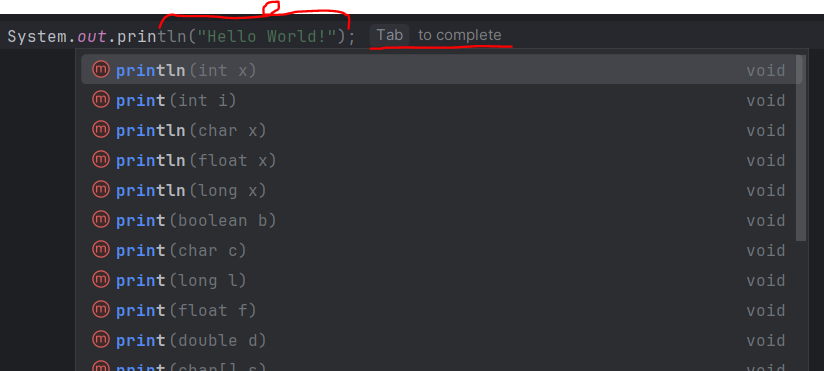
\includegraphics{img/AutocompleteIntelliJ.PNG}
    \end{center}
\end{enumerate}
\newpage


\aufgabe{Aufgabe 1: Variablen und Ausgaben}
Man kann mit System.out.println(einString) den Wert von einString in der Konsole (unten in der Mitte bei der Ausführung des Codes) ausgeben. Folgender code:
\begin{minted}{java}
System.out.println("PSE-Zeit ist Grillzeit")
\end{minted}
Gibt folgendes aus:
\begin{ausgabe}
    PSE-Zeit ist Grillzeit
\end{ausgabe}

\begin{enumerate}
    \item Kopiert folgenden Grill und nutzt print(s) um ihn in der Konsole auszugeben. 
    \begin{ausgabe}
.............................................................................
.............................................................................
...................................@.........................................
..................................\#@...-.....................................
..................................@@....@....................................
.................................@@@...@@....................................
.................................@@....@@....................................
................................@@-...@@.....................................
................................@@...@@-.....................................
................................@:...@@......................................
................................@....@.......................................
.................................=....\%......................................
.............................................................................
...................@@@@@@@@@@@@@@@@@@@@@@@@@@@@@@@@@@@.......................
....................@@@@@@@@@@@@@@@@@@@@@@@@@@@@@@@@@........................
....................\%@@@@@@@@@@@@@@@@@@@@@@@@@@@@@@@@@@@@....................
.....................@@@..@@@@@@@@@@@@@@@@@@@@@@@@@@@@@@.....................
.....................:@@@*.@@@@@@@@@@@@@@@@@@@@@@@@*.........................
......................-@@@@@@@@@@@@@@@@@@@@@@@@@@@\#..........................
........................@@@@@@@@@@@@@@@@@@@@@@@@@............................
..........................@@@@@@@@@@@@@@@@@@@@@-.............................
............................@@@@@@@@@@@@@@@@@................................
...............................@@@@@@@@@@@:..................................
..............................@@@-......@@@..................................
.............................@@@*........@@@.................................
............................@@@@..........@@@................................
...........................@@@@............@@@...............................
......................\#@@@@@@@.............:@@@..............................
....................@@@@@@@@@@..............+@@@.............................
...................=@@@@..@@@@@@@@@@@@@@@@@@@@@@@............................
...................@@@@....@@@@.:.............@@@*...........................
....................@@@@@@@@@@\#................@@@:..........................
.....................@@@@@@@@...................@@@..........................
.............................................................................
    \end{ausgabe}
    \item Erstelle eine Variable mit beliebigem Wert und gib sie aus, ändere den Wert und gib dieselbe Variable nochmal aus.
    \item Erstelle zwei int Variablen und gib die Summe und das Produkt aus.
    \item Erstelle eine Variable mit deinem Namen und schreibe genau ein Print, das dich mit deinem Namen begrüßt.
\end{enumerate}

\newpage
\aufgabe{Aufgabe 2: Scanner}
Man kann während das Program ausgeführt wird auch Werte aus der Konsole einlesen. Das geht mit einem Scanner Objekt. Mit scannerObjekt.next() wird die nächste eingegebene Zeile eingelesen. Mit \textbf{Enter} beendet man die Eingabe.  
\begin{minted}{java}
Scanner derScanner = new Scanner(System.in);
System.out.println("Gib deinen Namen ein:");
String deinName = derScanner.next();
System.out.println("Du heißt: " + deinName);
\end{minted}

\begin{enumerate}
    \item Programmier einen addierer, der zwei Zahlen einliest und die Summe ausgibt. Etwas funktioniert nicht, überlegt mal warum (Auflösung in der Fußnote
    \footnote{
        next() gibt einen String zurück, wenn man die beiden addiert werden die beiden Zahlen stumpf hintereinandergeschrieben, statt gescheit addiert zu werden. Dafür besitzt Scanner die nextInt() Funktion.
    }
    )?
    \item Programmier ein Modulo Trainer, bei dem man zwei Zahlen eingibt, dann das Ergebnis von zahl1 \% zahl2 eingeben soll und dann am Ende das korrekte Ergebnis ausgegeben wird.
\end{enumerate}

\newpage
\aufgabe{HIGHPERFORMER-Aufgabe: Zufallszahlen}
Java stellt einen Zufallszahlengenerator zur Verfügung. Dieser wird ähnlich wie Scanner benutzt und besitzt unter anderem folgende Funktionen:

\begin{minted}{java}
Random rndGenerator = new Random();

//gibt ein zufälligen float zwischen 0.0 und 1.0 zurück:
float zufallsFloat = rndGenerator.nextFloat();

//gibt ein zufälligen int zwischen 0 und 9 zurück (10 wird als Obergrenze ausgeschlossen)
int zufallsInt = rndGenerator.nextInt(10);
\end{minted}

\begin{enumerate}
    \item Modifiziere deinen Modulotrainer sodass man die beiden Zahlen nicht mehr selbst eingibt (war auch wirklich zu leicht so), sondern so, dass diese zufällig generiert werden. 
    \item In folgendem code bekommt ihr einen sogenannten Seed (5-Stellig) vom eingebauten Java Zufallsgenerator. Generiert mit den mathematischen Operatoren die ihr jetzt kennt anhand dieses Seeds eine neue 10-Stellige Zufallszahl. Wir (die PSE-Vorkurs Hauptorgas) haben ein Testerprogramm geschrieben, dass versucht eure Lösung zu bewerten und eventuelle Schwächen eures Ansatzes aufzuzeigen, doch vielleicht kriegt ihr es auch hin den Test auszutricksen.
    
    \begin{minted}{java}
public int zufallsZahl(int seed) {
    //seed ist die ursprüngliche 5-stellige Zahl mit der ihr rechnen könnt
    int rueckgabeZahl;

    // Schreibt euren code, der am ende eure neue zehnstellige Zahl
    // der Variable rueckgabeZahl zuweisen soll zwischen hier...


    // ... und hier
    return rueckgabeZahl
}
    \end{minted}
\end{enumerate}

\end{document}